%!TEX root = ..\..\main.tex
\chapter{Introduction}
\label{Ch:CouplingIntro}

\lhead{Chapter \ref{Ch:CouplingIntro}. \emph{Introduction}} % This is for the header on each page


\section{The Ising Model}
\label{sec:Ising}
	The Ising model is named after Ernst Ising who studied it in his 1924 thesis \cite{Ising1925-nd} under the supervision of Wilhelm Lenz who invented the model \cite{Lenz1920-bn}. It was originally motivated by the phenomenon of ferromagnetism but it has since been re-interpreted to apply to numerous other situations in both physics and other fields \footnote{See \cite[notes of Section 1.4.2]{Friedli2017-xm} for a list of references concerning this.}.

	The Ising model has enjoyed a prominent position in the statistical physics literature. This is largely due to the existence of a phase transition, a sharp transition in the large scale behaviour of the model as a parameter moves past a critical value. The transition was first shown to exist by Rudolph Peierls \cite{Peierls1936-pu} in what was the first proof of the existence of a phase transition for any model in statistical mechanics.
	Additionally, the Ising model is both relatively simple, and also mathematically tractable in some non-trivial cases \cite{Onsager1944-li}. These qualities are rare among models with a phase transition and so the Ising model has become somewhat of a staple for both studying phase transitions and testing new statistical mechanics techniques.

	The model is a probability distribution on spin configurations - assignments of $+1$ and $-1$ spins to each vertex in a finite graph $G = (V, E)$. The set of all possible configurations is
	\begin{equation}
		\Omega = \{-1, +1\}^V
	\end{equation}
	and for a particular configuration, $\sigma \in \Omega$, we refer to the spin of a particular vertex $i \in V$ with $\sigma[i]$. Each configuration has an associated energy, given by 
	\begin{equation}
		H_{G, \beta, h}(\sigma) = -\beta \sum_{ij \in E} \sigma[i] \sigma[j] - h\sum_{i \in V} \sigma[i]
	\end{equation}
	where $\beta \in [0, \infty)$ is the inverse temperature, and $h \in \mathbb{R}$ is the magnetic field. 

	The Gibbs measure is the distribution on $\Omega$ that characterises the Ising model and it is defined by
	\begin{equation}
		\pi_{G, \beta, h}(\sigma) \propto \exp(-H_{G, \beta, h}(\sigma)).
		\label{eq:gibbsmeasurefull}
	\end{equation}
	In everything that follows, we will be concerned only with the zero-field ($h = 0$) Ising model. This gives us the slightly simpler form for the Gibbs measure,
	\begin{equation}
		\pi_{G, \beta}(\sigma) \propto \exp \left( \beta \sum_{ij \in E} \sigma[i] \sigma[j] \right), \qquad \sigma \in \{-1, 1\}^V.
		\label{eq:gibbsmeasure}
	\end{equation}

	\subsection{The Phase Transition}
	An in depth study of the Ising phase transition and its associated critical temperature will not be needed for this work. However, we will still wish to refer to it occasionally and so here we give a workable description of the phase transition on lattices.

	Consider the Gibbs measure with zero-field \eqref{eq:gibbsmeasure} in the limits $\beta \downarrow 0$ and $\beta \uparrow \infty$. It is easy to see that in the former limit, the measure is uniform across all configurations and in the latter limit, the measure assigns all weight to the constant configurations $\sigma^- = (-1, -1, \dots, -1)$ and $\sigma^+ = (+1, +1, \dots, +1)$. This leads to the following overly simplistic description of the phase transition. It is the change in distribution that occurs as we increase the temperature; from distributions concentrated on states whose spins mostly agree, to distributions producing states which have roughly equal numbers of plus and minus spins.

	To be slightly more concrete we define quantities called the magnetization and magnetization density. The \emph{magnetization} on a volume $\Lambda \subseteq V$ is defined as 
	\begin{equation}
		M_\Lambda(\sigma) = \sum_{i \in \Lambda} \sigma[i].
	\end{equation}
	Normalizing this gives the \emph{magnetization density}, $M_\Lambda(\sigma)/|\Lambda|$. On the $d$-dimensional torus with side length $L$, $G(L) = (\mathbb{Z}/L\mathbb{Z})^d$, the quantity
	\begin{equation}
		L(\beta) = \lim_{L \rightarrow \infty} \expect_\beta \left|\frac{M_{G(L)}(\sigma)}{|G(L)|} \right|
		\label{eq:limitmagnetizationdensity}
	\end{equation}
	depends on the inverse temperature $\beta$. When $d = 1$, $L(\beta) = 0$ for any $\beta$ and there is no phase transition. However, when $d > 1$, there exists some critical $\beta_c(d)$ such that $L(\beta) = 0$ for $\beta < \beta_c(d)$ and $L(\beta) > 0$ for $\beta > \beta_c(d)$ \cite{Friedli2017-xm}. This $\beta_c(d)$ is the critical inverse temperature at which we observe a phase transition.

	% On most graphs [FIND OUT WHICH] the Ising model undergoes a phase transition at a critical inverse temperature $\beta_c = \beta_c(G)$ that is dependent on the graph. Roughly speaking, for $\beta < \beta_c$ (the high-temperature regime), the correlation of spins dies off quickly with the distance between them and for $\beta > \beta_c$ (the low-temperature regime), spins remain correlated at a large distance.

	% [EXTEND]

\section{Coupling from the Past}
	One of the primary concerns regarding the Ising model is how to efficiently sample from the Gibbs measure. Calculating the normalizing constant for \eqref{eq:gibbsmeasure}, known as the partition function, is a \#P-complete problem \cite{Jerrum1993-ii}. As such a direct approach to sampling is computationally intractable and so other methods must be employed instead. One such method is Markov Chain Monte Carlo (MCMC). This involves constructing a Markov chain whose states are elements of $\Omega$ and whose stationary distribution is given by \eqref{eq:gibbsmeasure}. One can then obtain a sample by running this Markov chain for long enough that the output has distribution sufficiently close to \eqref{eq:gibbsmeasure}.
	% The zero-field ferromagnetic Ising model on finite graph $G = (V, E)$ at 
	% inverse temperature $\beta \geq 0$ has Gibbs measure
	%
	One difficulty in using MCMC is that, initially, one does not know how long to run the chain for. In principal, bounds on this time can be achieved, but in practise, proving these bounds can be very challenging.

	An alternative to MCMC was introduced by Propp and Wilson called Coupling from the Past (CFTP) \cite{Propp1996-cf}. Unlike MCMC, CFTP not only has an automatically determined running time, but it has the additional advantage of outputting exact samples from the stationary distribution. This does not come without a cost - CFTP has a random running time. Therefore, a key question towards evaluating the effectiveness of CFTP is understanding the distribution of its running time, that is, the \emph{coupling time}.

	In Chapters \ref{Ch:1D} and \ref{Ch:GeneralResults}, we will investigate the coupling time for the Ising heat-bath Glauber dynamics, both on the cycle, at any temperature, in Chapter \ref{Ch:1D}, and on any vertex transitive graph, at sufficiently high temperatures, in Chapter \ref{Ch:GeneralResults}. Our main result in each chapter will be proving that, when appropriately scaled, the coupling time essentially converges to a Gumbel distribution as the size of the graph increases. 

	\subsection{Ising heat-bath Glauber dynamics}
	\label{sec:heat-bath glauber dynamics definition}
	The continuous-time heat-bath Glauber dynamics for the Ising model is a Markov chain whose states are elements of $\Omega$ and whose stationary distribution is given by \eqref{eq:gibbsmeasure}. For a given graph $G = (V, E)$, and a given inverse temperature, $\beta$, we can describe the dynamics as follows. 

	Initialize every vertex in $V$ with a spin (for example, we could start in the all-plus configuration). To each vertex in $V$ we give an i.i.d.\ rate-one Poisson clock. Define the probability 
	\begin{equation}
		p_i(\sigma) = \frac{\euler^{\beta S_i(\sigma)}}{\euler^{\beta S_i(\sigma)} + \euler^{-\beta S_i(\sigma)}}
		\label{eq:define p_i}
	\end{equation}
	where
	\begin{equation}
		S_i(\sigma) = \sum_{j \sim i} \sigma[j]
	\end{equation}
	is the sum of the spins of the neighbours of $i$, and $j \sim i$ denotes that $j$ is connected to $i$ with some edge $ij \in E$. Let $\sigma_t$ denote the spin configuration at time $t$. When the clock of vertex $i$ rings at some time $t$, we update $\sigma_t[i]$ to $+1$ with probability $p_i(\sigma_t)$, and to $-1$ otherwise.

	\subsection{The Coupling Time}
	\label{sec:the coupling time}
	We now describe the two coupled chains from which we define the coupling time of the Ising heat-bath Glauber dynamics. In order to do this, it will prove convenient to use a random mapping representation for the jump process. This will also help us outline an implementation of CFTP for our coupling.

	Define $f: \Omega \times V \times [0,1] \mapsto \Omega$ via $f(\sigma, i, u) = \sigma'$ where $\sigma'[j] = \sigma[j]$ for $j \neq i$ and
	\begin{equation}
		\sigma'[i] = 
			\begin{cases}
				1, &u \leq p_i(\sigma),\\
				-1, &u > p_i(\sigma).
			\end{cases}
		\label{eq:plusorminusrules}
	\end{equation}
	Let $\mathscr{V}$ and $U$ be independent, with $\mathscr{V}$ uniform on $V$ and $U$ uniform on $[0,1]$. Then, updating our chain at rate $n = |V|$, and performing updates from $\sigma$ to $\sigma'$ according to $\sigma' = f(\sigma, \mathscr{V}, U)$, we recover the dynamics described in Section \ref{sec:heat-bath glauber dynamics definition}.

	We also note that $f$ is monotonic, in the following sense. We define a partial ordering on $\Omega$ by writing that $\sigma \preceq \omega$ if $\sigma, \omega \in \Omega$ are such that $\sigma[i] \leq \omega[i]$ for all $i \in V$ (and similarly for $\sigma \succeq \omega$). Then for any fixed $i \in V$ and $u \in [0,1]$, if $\sigma \preceq \omega$ then $f(\sigma, i, u) \preceq f(\omega, i, u)$.
	
	Let $(\mathscr{V}_k, U_k)_{k \geq 1}$ be an i.i.d. sequence of copies of $(\mathscr{V}, U)$. Define top and bottom chains, $(\mathscr{T}_t)_{t\geq0}$ and $(\mathscr{B}_t)_{t\geq0}$, with initial states
	\begin{align}
		\mathscr{T}_0 &= (1, 1, \dots, 1)\\
		\mathscr{B}_0 &= (-1, -1, \dots, -1)
	\end{align}
	that update together at rate $n$. On the $k$th update at time $t_k$, update $\mathscr{T}_{t_k}$ to $f(\mathscr{T}_{t_k}, \mathscr{V}_k, U_k)$ and update $\mathscr{B}_{t_k}$ to $f(\mathscr{B}_{t_k}, \mathscr{V}_k, U_k)$.

	We call the coupled process, $(\mathscr{B}_t, \mathscr{F}_t)_{t\geq0}$, \emph{the Ising heat-bath coupling}. From the monotonicity of $f$, $\mathscr{T}_t \succeq \mathscr{B}_t$, for all $t \geq 0$.

	A more descriptive explanation of the coupling is that the top and bottom chains share the same rate-one Poisson clocks at each vertex, and upon updating that vertex, we share the same uniform random variable $U$ between the two chains to determine whether to update to a plus or minus according to \eqref{eq:plusorminusrules}.

	The \emph{coupling time} of the Ising heat-bath process is the random variable
	\begin{equation}
		T = \inf \left\{t : \mathscr{T}_t = \mathscr{B}_t \right\}.	
	\end{equation}
	This is the main object of interest for our analysis. Note that the coupling time is not just a property of the Ising heat-bath process, but also of the coupling we have chosen. In Section \ref{sec:information percolation on the cycle} we will make a change to the coupling we use to make the analysis easier. Some care will need to be taken to verify that the coupling time is not affected by this change.

	\subsection{Equivalence of Discrete and Continuous Coupling Time}
	So far we have stated that the running time of CFTP has the same distribution as the coupling time. In fact, we have glossed over one important detail. Namely, CFTP is exclusively run in discrete time, and our coupling time is defined by the continuous time dynamics. Therefore, for our motivation to be reasonable, we would like to show some sort of equivalence between the distributions of the discrete and continuous coupling times. We do this via Claim \ref{claim:discrete vs continuous distributions}.

	\begin{claim}
	\label{claim:discrete vs continuous distributions}
		Let $(N_n)_{n \in \mathbb{N}}$ be a sequence of positive random variables, and $(a_n)_{n \in \mathbb{N}}$ be a non-decreasing sequence of integers such that $N_n \geq a_n$ for all $n$ and $\lim_{n \rightarrow \infty} a_n = \infty$.	Define $T(n)$ be the random time it takes for a rate $\lambda$ Poisson clock to go off $n$ times (this is the time it takes for $n$ updates to occur in a continuous-time Markov Chain).

		Assume there exists a deterministic sequence $w_n$ and constant $C$ such that either
		\begin{equation}
			\lim_{n\rightarrow \infty} \prob\left[\left|\frac{T(N_n)}{w_n}\right| > C\right]  = 0,
			\label{eq:Y_n goes to zero}
		\end{equation}
		or 
		\begin{equation}
			\lim_{n\rightarrow \infty} \prob\left[\left|\frac{N_n}{\lambda w_n}\right| > C\right]  = 0.
			\label{eq:Z_n goes to zero}
		\end{equation}
		Then
		\begin{equation}
			\lim_{n \rightarrow \infty} \prob(T(N_n) < w_n) = L
			\label{eq:limit CT is L}
		\end{equation}	
		if and only if
		\begin{equation}
			\lim_{n \rightarrow \infty} \prob(N_n < \lambda w_n) = L.
			\label{eq:limit DT is L}
		\end{equation}
	\end{claim}
	\begin{proof}
		By the triangle inequality,
		\begin{align}
			|\prob(N_n < \lambda w_n) - L| &\leq \left|\prob(N_n < \lambda w_n) - \prob\left(T(N_n) < w_n\right)\right| + \\
				&\phantom{\leq \,} \left|\prob\left(T(N_n) < w_n\right) - L\right| \notag
		\end{align}
		and also
		\begin{align}
			\left|\prob\left(T(N_n) < w_n\right) - L\right| &\leq \left|\prob(N_n < \lambda w_n) - \prob\left(T(N_n) < w_n\right)\right| + \\
				&\phantom{\leq \,}|\prob(N_n < \lambda w_n) - L|.  \notag
		\end{align}

		From \eqref{eq:limit CT is L} and \eqref{eq:limit DT is L}, the latter terms in each of the above inequalities vanish in the limit. Therefore, the key to both directions of the proof is to show that
		\begin{equation}
			\left|\prob(N_n < \lambda w_n) - \prob\left(T(N_n) < w_n\right)\right| = \left|\prob\left(Z_n < 1\right) - \prob\left(Y_n < 1\right)\right|
		\end{equation}
		vanishes as $n \rightarrow \infty$. (We have introduced $Y_n = T(N_n)/w_n$ and $Z_n = N_n/(\lambda w_n)$ for ease of notation). To do this it will be sufficient to show that the limiting distributions of $Y_n$ and $Z_n$ are equal.

		Note that $T(n)$ is the sum of $n$ i.i.d. exponential random variables with rate $\lambda$. It follows at once that
		\begin{align}
			\expect\left[T(n)\right] &= \frac{n}{\lambda},
			&\var\left[T(n)\right] &= \frac{n}{\lambda^2}.
		\end{align}
		Hence
		\begin{align}
			\expect\left[\frac{\lambda T(n)}{n}\right] &= 1,
			&\var\left[\frac{\lambda T(n)}{n}\right] &= \frac{1}{n}.
		\end{align}
		Now since $N_n \geq a_n$, for any $\epsilon > 0$,
		\begin{align}
			\prob\left(\left|\frac{\lambda T(N_n)}{N_n} - 1\right| \geq \epsilon\right) &\leq \prob\left(\left|\frac{\lambda T(a_n)}{a_n} - 1\right| \geq \epsilon\right).\\
			&\leq \frac{1}{a_n \epsilon^2}
			\label{eq:Y_n/Z_n - 1 goes to 0}
		\end{align}
		where the last line comes from Chebyshev's inequality.

		Then, for any $\epsilon > 0$, and for some $C \in \mathbb{R}$,
		\begin{align}
			\prob\left(\left|Y_n - Z_n\right| \geq C \epsilon \right) &= \prob\left(\left|\frac{Y_n}{Z_n} - 1\right| \geq \frac{C}{|Z_n|} \epsilon \right)\\
			&=  \prob\left(\left. \left|\frac{Y_n}{Z_n} - 1\right| \geq \frac{C}{|Z_n|} \epsilon \, \right| |Z_n| \leq C \right) \prob(|Z_n| \leq C) \notag \\
			&\phantom{=}+  \prob\left(\left. \left|\frac{Y_n}{Z_n} - 1\right| \geq \frac{C}{|Z_n|} \epsilon \, \right| |Z_n| > C \right) \prob(|Z_n| > C)\\
			&\leq \prob\left(\left|\frac{Y_n}{Z_n} - 1\right| \geq \epsilon \right) + \prob(|Z_n| > C).
		\end{align}
		If \eqref{eq:Z_n goes to zero} holds then we are done. Otherwise, note that if $|Y_n| \leq C/2$ and $|Y_n/Z_n - 1| \leq 1/2$, then $|Z_n| \leq C$. So
		\begin{equation}
			\prob(|Z_n| > C) \leq \prob(|Y_n| > C/2) + \prob\left(\left|\frac{Y_n}{Z_n} - 1\right| > \frac{1}{2}\right)
		\end{equation}
		and overall
		\begin{equation}
			\prob(|Y_n - Z_n| \geq C\epsilon) \leq \prob\left(\left|\frac{Y_n}{Z_n} - 1\right| \geq \epsilon \right) + \prob(|Y_n| > C/2) + \prob\left(\left|\frac{Y_n}{Z_n} - 1\right| > \frac{1}{2}\right)
		\end{equation}
		% \begin{align}
		% 	\prob\left(\left|\frac{Y_n}{Z_n} - 1\right| \geq \epsilon_n\right)
		% 	&= \prob\left(|Y_n - Z_n| \geq |Z_n| \epsilon_n \right)\\
		% 	&= \prob\left(|Y_n - Z_n| \geq |Z_n| \epsilon_n \right | Z_n < C)\prob(Z_n < C) \notag \\
		% 	&\phantom{=} +  \prob\left(|Y_n - Z_n| \geq |Z_n| \epsilon_n \right | Z_n \geq C)\prob(Z_n \geq C)\\
		% 	&\leq \prob\left(|Y_n - Z_n| \geq C \epsilon_n \right | Z_n < C) + p_n\\
		% 	&\leq \frac{1}{(1 - p_n)a_n \epsilon_n^2} + p_n
		% \end{align}
		which, from \eqref{eq:Y_n goes to zero} and \eqref{eq:Y_n/Z_n - 1 goes to 0}, goes to zero. Hence $Y_n$ and $Z_n$ converge in probability, and hence they converge in distribution as required.
	\end{proof}

	Often the sequence $w_n$ of Claim \ref{claim:discrete vs continuous distributions} is of the form $w_n = w_n(z) = a_n z + b_n$ and we have that 
	\begin{equation}
		\lim_{n\rightarrow \infty} \prob(T_n \leq w_n(z)) = G(z)
	\end{equation}
	for some distribution $G(z)$. The following Lemma shows that if this is the case, in order for either \eqref{eq:Y_n goes to zero} or \eqref{eq:Z_n goes to zero} to hold, it is enough that $b_n$ dominates $a_n$.

	\begin{lemma}
	\label{lem: a_n/b_n goes to infty is enough}
		If there exists sequences $a_n$ and $b_n$ such that $b_n/a_n \rightarrow \infty$ and
		\begin{equation}
			\prob\left(T_n < a_n z + b_n\right) \rightarrow G(z)
		\end{equation}
		for some distribution function $G(z)$, then for all $C > 1$,
		\begin{equation}
			\lim_{n \rightarrow \infty} \prob\left(\frac{T_n}{a_n z + b_n} > C\right) = 0.
		\end{equation}
	\end{lemma}
	\begin{proof}
		First observe that
		\begin{align}
			\prob\left(\frac{T_n}{a_n z + b_n} \leq C\right) &= \prob\left(T_n \leq C(a_n z + b_n)\right)\\
			&= \prob\left(T_n \leq a_n(Cz + (C - 1) b_n/a_n) + b_n \right).
		\end{align}
		Since $b_n / a_n \rightarrow \infty$, and $C > 1$, for any $x\in \mathbb{R}$, there exists an $M \in \mathbb{N}$ such that for all $n > M$,
		\begin{equation}
			\prob\left(T_n \leq a_n(Cz + (C - 1) b_n/a_n) + b_n \right) \geq \prob\left(T_n \leq a_n x + b_n\right).
		\end{equation}
		Hence for all $x \in \mathbb{R}$,
		\begin{equation}
			\lim_{n\rightarrow \infty} \left(\frac{T_n}{a_n z + b_n} \leq C\right) \geq G(x)
		\end{equation}
		and since $G(x)$ is a distribution
		\begin{equation}
			\lim_{n\rightarrow \infty} \left(\frac{T_n}{a_n z + b_n} \leq C \right) = 1
		\end{equation}
	\end{proof}

	\begin{remark}
		We apply Claim \ref{claim:discrete vs continuous distributions} to the coupling time of the Glauber heat-bath dynamics in the following way. Take $N_n$ to be the discrete coupling time on a graph of size $n$. The continuous time coupling time is given by $T(N_n)$. Note that $N_n \geq n$ since each vertex must be updated at least once for coupling to occur. From Lemma \ref{lem: a_n/b_n goes to infty is enough} along with Theorems \ref{thm:Coupling Distribution on Cycle} and \ref{thm:Coupling Distribution on Lattice} we get that \eqref{eq:Y_n goes to zero} is satisfied. This means that, appropriately scaled, the discrete-time coupling time has the same limiting distribution as the continuous-time coupling time.
	\end{remark}

	\subsection{Summary of CFTP}
	\label{sec:summary of CFTP}
	We are now in a position to give a brief summary of the CFTP method, as it applies to the Ising heat-bath coupling. It should be noted that we include this summary of CFTP for completeness. None of the details regarding the implementation of CFTP are required outside of this section. It serves only as motivation for the study of the coupling time.

	Let $f: \Omega \times V \times [0,1] \mapsto \Omega$ and $(\mathcal{V}, U)$ be as defined in Section \ref{sec:the coupling time}. Let $(\mathcal{V}_k, U_k)$ be an i.i.d. sequence of copies of $(\mathcal{V}, U)$ and define 
	\begin{equation}
		f_{-k} = f(\cdot, \mathcal{V}_k, U_k).
	\end{equation}
	We construct the composition
	\begin{equation}
		F_{-k} = f_0 \circ f_1 \circ \dots \circ f_{k-1}
	\end{equation}
	and define the \emph{backwards coupling time} to be
	\begin{equation}
		T_\mathrm{BACK} = \min\{k \in \mathbb{N} : F_{-k}(\mathscr{B}_0) = F_{-k}(\mathscr{T}_0)\}.
	\end{equation}

	The state $F_{-T_\mathrm{BACK}}(\mathscr{B}_0) = F_{-T_\mathrm{BACK}}(\mathscr{T}_0)$ is the output of the CFTP algorithm, and was shown by Propp and Wilson \cite{Propp1996-cf} to be an exact sample from the chain's stationary distribution. To see why this is so, observe that by the monotonicity of $f$, if $F_{-k}(\mathscr{B}_0) = F_{-k}(\mathscr{T}_0)$, then $F_{-k}(\sigma) = F_{-k}(\mathscr{B}_0)$ for any $\sigma \in \Omega$. If we let $\sigma_\pi$ be a random sample from the stationary distribution $\pi$, then $F_{-k}(\mathscr{B}_0) = F_{-k}(\mathscr{T}_0) = F_{-k}(\sigma_\pi)$ must also have distribution $\pi$, which in our case is given by \eqref{eq:gibbsmeasure}.
	
	If we reverse the composition to construct
	\begin{equation}
		F_{k} = f_{k} \circ f_{k-1} \circ \dots \circ f_1
	\end{equation}
	we can define the usual discrete time coupling time as
	\begin{equation}
		T_\mathrm{DIS} =  \min\{k \in \mathbb{N} : F_{k}(\mathscr{B}_0) = F_{k}(\mathscr{T}_0)\}.
	\end{equation}
	The forwards coupling time, $T_\mathrm{DIS}$, has the same distribution as the backwards coupling time, $T_\mathrm{BACK}$, although in general, $F_{T_\mathrm{DIS}}(\mathscr{B}_0) = F_{T_\mathrm{DIS}}(\mathscr{T}_0)$ does not have distribution \eqref{eq:gibbsmeasure}.

	In practise, one runs the CFTP algorithm by starting both the top and bottom chains from some point in the past to time zero. This is repeated for increasingly more distant times in the past until both chains agree at time 0. The sequence of times at which one restarts this process need not be $-1, -2, -3, \dots$, rather, any monotonic natural sequence $a_1, a_2,\dots$ can  be used. See \cite{Levin2009-fo}, \cite{Haggstrom2002-os}, and \cite{Jerrum1998-ph} for further discussion.

	
\section{Information percolation}
	A cornerstone to the proofs contained in Chapters \ref{Ch:1D} and \ref{Ch:GeneralResults} is the framework of information percolation, first introduced by Lubetzky and Sly in 2016 \cite{Lubetzky2016-wd}. In this paper, Lubetzky and Sly managed to achieve much sharper results, in much more generality, regarding the mixing time for the Glauber dynamics for the Ising model than had been achieved before. In this section we provide a brief summary of their paper before laying out the basic framework, in the context of the Ising heat-bath dynamics, that will be required for Chapters \ref{Ch:1D} and \ref{Ch:GeneralResults}.

	\subsection{Information percolation and cutoff for the stochastic Ising model}
	In order to define cutoff, the central phenomenon of study in Lubetzky and Sly's 2016 paper titled, `Information percolation and cutoff for the stochastic Ising model', we first have to define the total-variation mixing time. Given a parameter $\epsilon$, a Markov Chain $Y_t$ has mixing time
	\begin{equation}
		t_\mathrm{MIX}(\epsilon) = \inf\left\{t: \max_{x_0 \in \Omega} ||\prob(X_t \in \cdot | X_0 = x_0) - \pi ||_\mathrm{TV} \leq \epsilon \right\}
	\end{equation}
	where the total variation distance $||\nu_1 - \nu_2||_\mathrm{TV}$ is defined as 
	\begin{equation}
		\max_{A \in \Omega}|\nu_1(A) - \nu_2(A)| = \frac{1}{2}\sum_{\sigma \in \Omega} |\nu_1(\sigma) - \nu_2(\sigma)|.
	\end{equation}
	A family of Markov chains $(Y_t)$ indexed by $n$ is said to exhibit cutoff if
	\begin{equation}
		t_\mathrm{MIX}(\epsilon) = (1 + o(1)) t_\mathrm{MIX}(\epsilon'),
	\end{equation}
	for any fixed $0 < \epsilon, \epsilon' < 1$. A \emph{cutoff window} is a sequence $w_n$ where
	\begin{equation}
		t_\mathrm{MIX}(\epsilon) = t_\mathrm{MIX}(1 - \epsilon) + \mathcal{O}(w_n)
	\end{equation}
	for any $0 < \epsilon <1$.

	Historically, proving cutoff has proven to be highly challenging. In a survey on the topic, Diaconis \cite{Diaconis1996-sz} wrote `proof of a cutoff is a difficult, delicate affair, requiring detailed knowledge of the chain, such as all eigenvalues and eigenvectors'. It is therefore worth noting the significant gap between the strength of the results regarding cutoff achieved using information percolation, and those that existed previously.

	Previous to \cite{Lubetzky2016-wd}, the best result known for general graphs was that cutoff occurs with a $\mathcal{O}(1)$ window in the simple case when $\beta = 0$ \cite{Aldous1983-gz}. However, no results were known for $\beta > 0$, despite a conjecture by \citeauthor{Levin2009-fo} in 2009 \cite[Section 23.2]{Levin2009-fo} that cutoff occurs on any sequence of transitive graphs when the mixing time is of order $\log n$ (as one would expect when $\beta < c_0$ for some $c_0 > 0$ that depends on the sequence of graphs). On lattices, the first results to appear were due to Lubetzky and Sly in 2013 who established cutoff up to the critical temperature for dimensions $d \leq 2$ with only a $\mathcal{O}(\log \log n)$ window \cite{Lubetzky2013-yv}. 

	Using information percolation, Lubetzky and Sly proved the existence of cutoff for the continous time Glauber dynamics for the Ising model with an $\mathcal{O}(1)$ window on $\mathbb{Z}^d$ for all temperatures up to the critical temperature. In a companion paper \cite{Lubetzky2017-nc}, they extended this result to include any graph for sufficiently high temperature. Since these papers, information percolation has also been used to establish cutoff for the Swendsen-Wang dynamics on the lattice \cite{Nam2018-io}, suggesting that the technique is effective on a broader class of problems than simply Glauber dynamics for Ising.
	
	\subsection{The framework}
	At its core, information percolation is a way of tracking how the dependencies of the final spins of the Glauber heat-bath dynamics percolate through the graph over time. These dependencies are traced backwards through time from some designated time $t^*$ on the space-time slab $V \times [0, t^*]$ (see Figure \ref{fig:typical percolation} for example) to create the update history. These histories are made in such a way so that, if for any $j \in V$ no path exists connecting $(i, t^*)$ to $(j, 0)$, then the spin of $i$ does not depend on the initial state (and thus at time $t^*$ vertex $i$ takes $+1$ and $-1$ spins with equal probability by symmetry). The main constructs used to create this history are the update sequence, and the update support function which we will now define.

	\begin{figure}[ht]
		\centering
		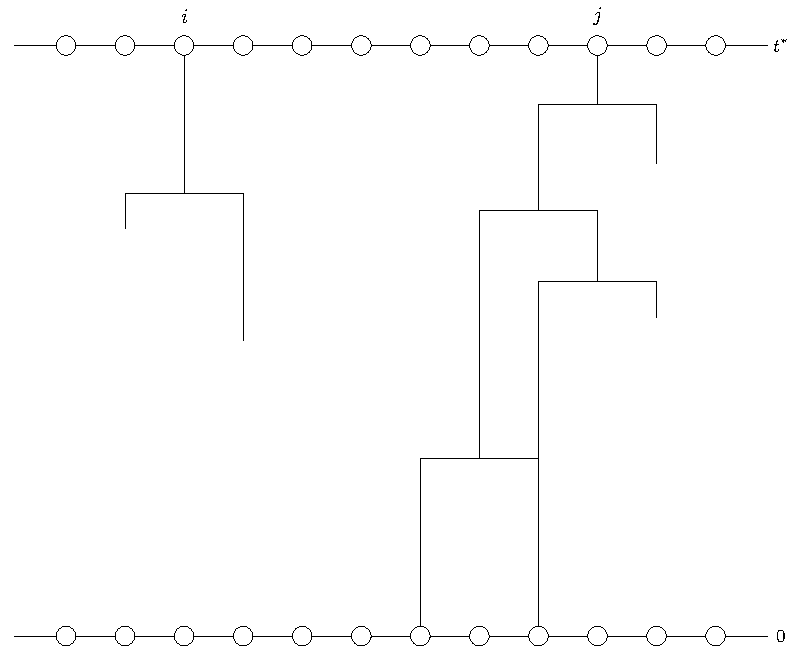
\includegraphics[width = \textwidth]{Figures/IsingCouplingTime/typical_percolation.pdf}
		\caption{A section of the space-time slab $V \times [0, t^*]$ along with a typical appearance of the update histories for two vertices on the cycle. Time runs vertically from bottom to top, and the vertices are represented by circles, laid out horizontally. If there is a path in the update history of $v$ between points $(u, t)$ and $(v, t^*)$, then the spin of $v$ at time $t^*$ depends on the spin of $u$ at time $t$. In this example, since there is no path from vertex $(i, t^*)$ to time $0$, the final spin at $i$ does not depend on the initial configuration whereas the final spin at $j$ does.}
		\label{fig:typical percolation}
	\end{figure}

	\subsubsection{The update sequence}
	Recalling our random mapping representation from Section \ref{sec:the coupling time}, we can encode an update of our coupled process with the tuple $(\mathcal{V}, U, t)$, where $t$ is the time of the update, $\mathcal{V}$ is the vertex that is updated, and $U$ is the value of the uniform random variable that tells us whether $\mathcal{V}$ is a plus or minus according to \eqref{eq:plusorminusrules}. The \emph{update sequence} along an interval $(t_0, t_1]$ is the set of these tuples with $t_0 < t \leq t_1$. Given the state of our Markov Chain at time $t_0$, $Y_{t_0}$, the update sequence along $(t_0, t_1]$ contains all the information we need to contruct $Y_{t_1}$. In particular, given the update sequence along the interval $(0, t_1]$, $Y_{t_1}$ is a deterministic function of $Y_0$.

	\subsubsection{The update support function}
	\label{sec: definition update support function}
	Given the update sequence along the interval $(t_1, t_2]$, the \emph{update support function}, $\mathscr{F}(A, t_1, t_2)$, is the minimal set of vertices whose spins at time $t_1$ determine the spins of the vertices in $A$ at time $t_2$. That is, $i \in \mathscr{F}(A, t_1, t_2)$ if and only if there exist states $Y_{t_1}, Y_{t_1}' \in \{-1, +1\}^{V}$ that differ only at $i$ and such that when we construct $Y_{t_2}$ and $Y_{t_2}'$ using the update sequence, $Y_{t_2} \neq Y_{t_2}'$.

	In particular, if $\mathscr{F}(i, 0, t) = \emptyset$ then the spin at vertex $i$ at time $t$ does not depend on the initial state and so for any two coupled chains $Y$ and $Y'$, $Y_t[i] = Y_t'[i]$. 
	% It follows that
	% \begin{equation}
	% 	\prob \left[ Y_t[v] \neq Y_t'[v] \right] \leq \prob \left[ \mathscr{F}(v, 0, t) \neq \emptyset \right].
	% 	\label{eq:boundXneqY}
	% \end{equation}
	As a consequence of the monotonicity of our coupling, we can make the stronger statement that $\mathscr{T}_t[i] = \mathscr{B}_t[i]$ if and only if $\mathscr{F}(i, 0, t) = \emptyset$ which of course means that
	\begin{equation}
	\label{eq:prob equality of coupling and empty support}
		\prob[\mathscr{T}_t[i] \neq \mathscr{B}_t[i]] = \prob[\mathscr{F}(i, 0, t) \neq \emptyset].
	\end{equation}

	For ease of notation, we will often use the shorthand
	\begin{equation}
		\mathcal{H}_i(t) := \mathscr{F}(i, t, t^*).
	\end{equation}
	where $t^*$ is some target time that should be clear from context. We call this the \emph{update history of vertex $i$ at time $t$}. Tracing $\mathcal{H}_i(t)$ backwards in time from $t^*$ produces a subgraph of $\Omega \times [0, t^*]$ which we write as $\mathcal{H}_i$ and which we simply call the \emph{update history of vertex $i$}. To be slightly more precise, to produce $\mathcal{H}_i$ we connect $(j,t)$ to $(j,t')$ if $j \in \mathcal{H}_i(t)$ and there are no updates of $j$ along $(t', t]$ and we connect $(j,t)$ to $(j',t)$ if there was an update at $(j, t)$, $j \in \mathcal{H}_i(t)$, $j' \notin \mathcal{H}_i(t)$, and $j' \in \mathcal{H}_i(t+\epsilon)$ for any sufficiently small $\epsilon > 0$.

	% ALSO DEFINE UPDATE SUPPORT
	

	[USE FIGURE HERE TO MAKE CLEAR]
	To give some intuition to the definitions above, consider how we might construct the update history of a vertex $i$ from some target time $t^*$. We have at our disposal the update sequence along $(0, t^*]$ which we place in order of decreasing time. If vertex $i$ does not appear in the update sequence then we create a temporal edge between $(i, t^*)$ and $(i, 0)$ and our update history is complete - vertex $i$ was never updated and so it simply takes its initial value. Otherwise, we create temporal edge between $(i, t^*)$ and $(i, t_i)$ where $t_i$ is the last time vertex $i$ was updated. At this point we note from \eqref{eq:plusorminusrules} that the spin that vertex $i$ takes due to this update depends on the spins of its neighbours. So we add spatial edges from $(i, t_i)$ to $(j, t_i)$ for each $j\sim i$. Finally, we can iterate this process for each neighbour until every history has reached time $0$.

	This construction certainly contains every vertex that might influence the final spin at $i$, that is, it contains $\mathcal{H}_i$ as a subgraph. However, it is possible for updates to occur that do not depend on neighbouring spins. These updates cause temporal edges leading up to them to terminate without branching out to the neighbouring vertices. These type of updates are called \emph{oblivious updates}.

	\subsubsection{Oblivious updates}

	Generally speaking, an update to a vertex is oblivious if we do not need to know the configuration of its neighbours to determine the spin of that vertex. More precisely, an update, $(\mathcal{V}, U, t)$, is oblivious if 
	%for any $\sigma_1, \sigma_2 \in \Omega$, $\sigma_1' = f(\sigma_1, \mathcal{V}, U)$ and $\sigma_2' = f(\sigma_2, \mathcal{V}, U)$ are such that
	% \begin{equation}
	% 	\sigma_1'[\mathcal{V}] = \sigma_2'[\mathcal{V}].
	% \end{equation}
	\begin{equation}
		f(\sigma, \mathcal{V}, U)[\mathcal{V}] = f(\sigma', \mathcal{V}, U)[\mathcal{V}]
	\end{equation}
	for all $\sigma, \sigma' \in \Omega$, where $f$ is as defined in \eqref{eq:plusorminusrules}.

	Consider how these updates occur under our random mapping representation. Let $\Delta_i$ denote the degree of a vertex $i$. Recalling \eqref{eq:define p_i},
	\begin{equation}
		\frac{\euler^{-\beta \Delta_i}}{\euler^{\beta \Delta_i} + \euler^{-\beta \Delta_i}} \leq p_i(\sigma) \leq \frac{\euler^{\beta \Delta_i}}{\euler^{\beta \Delta_i} + \euler^{-\beta \Delta_i}},
	\end{equation}
	with equality holding for the lower and upper limits when the neighbours have spins all minus and all plus respectively. So for a particular update $(\mathcal{V}, U, t)$, if $U \leq \frac{\euler^{-\beta \Delta_\mathcal{V}}}{\euler^{\beta \Delta_\mathcal{V}} + \euler^{-\beta \Delta_\mathcal{V}}}$ then $\mathcal{V}$ is updated to a plus regardless of the configuration of its neighbours. Hence $(\mathcal{V}, U, t)$ is an oblivious update. Similarly, if $U > \frac{\euler^{\beta \Delta_\mathcal{V}}}{\euler^{\beta \Delta_\mathcal{V}} + \euler^{-\beta \Delta_\mathcal{V}}}$ then $\mathcal{V}$ is updated to a minus regardless of the configuration of its neighbours and hence $(\mathcal{V}, U, t)$ is an oblivious update. It is easy to see that these are the only types of oblivious updates.
	
	The rate of these updates at vertex $i$ is
	\begin{align}
		\theta_i &= 1 - \left(\frac{\euler^{\beta \Delta_i}}{\euler^{\beta \Delta_i} + \euler^{-\beta \Delta_i}} - \frac{\euler^{-\beta \Delta_i}}{\euler^{\beta \Delta_i} + \euler^{-\beta \Delta_i}}\right)\\
			&= 1 - \tanh(\beta \Delta_i).
	\end{align}
	If $G$ is a $\Delta$-regular graph (as will be the case in the following chapters) then we can drop the subscript and write $\theta = 1 - \tanh(\beta \Delta)$ for the rate of oblivious updates at each vertex.

	As noted earlier, oblivious updates cause temporal edges leading up to them in the update history to terminate. If $j \in \mathcal{H}_i(t)$, then an oblivious update $(j, u, t)$ removes $j$ from $\mathcal{H}_i(t)$ without adding any of its neighbours. It is worth remarking that these are not necessarily the only updates that can shrink the size of the update history of $i$ [FIGURE?]. However, for our analysis they will be the only such updates we will be concerned with. Indeed, in Chapter \ref{Ch:1D} we will use a different coupling so that these are the only updates that shrink the size of the update history, and in Chapter \ref{Ch:GeneralResults} we will use an alternative construction that bounds the true update history, in which updates are either oblivious or branch out to all $\Delta$ neighbours.

	

